\documentclass[12pt, titlepage]{article}
\usepackage[USenglish]{babel}
\usepackage[utf8]{inputenc}
\usepackage{amssymb, amsmath}
\usepackage{bm}
\usepackage{color}
\usepackage[unicode]{hyperref}
\usepackage{url}
\hypersetup{
    colorlinks,
    citecolor=blue,
    filecolor=blue,
    linkcolor=blue,
    urlcolor=blue
}
\usepackage{graphicx}
\usepackage{grffile}
\usepackage{listings}
\usepackage{float}

\def\sgn{\operatorname{sgn}}
\title{LinUCB vs HybridLinUCB}
\date{\today}
\author{Radek Bartyzal}

\begin{document}
\begin{titlepage}
    \centering
    \vfill
    {\bfseries\Huge
        LinUCB vs HybridLinUCB in recommender systems
    }    
    \vfill
        
    
        
    {\bfseries\Large 
    Author:\\
    Radek Bartyzal (bartyrad@fit.cvut.cz)\\
    }    
    \vskip1cm
 
    \vskip1cm
    \today

    
    \vfill
\end{titlepage}

\tableofcontents
\pagebreak

\section{Introduction}\label{sec:intro}
The algorithms LinUCB and HybridLinUCB are both introduced in the article A Contextual-Bandit Approach to
Personalized News Article Recommendation published in 2012.

The authors decided to model personalized recommendation of news
articles as a contextual bandit problem, a principled approach in
which a learning algorithm sequentially selects articles to serve
users based on contextual information about the users and articles,
while simultaneously adapting its article-selection strategy.

\section{Theory}\label{sec:theory}
Both algorithms are based on upper con-
fidence bound algorithm (UCB) that uses a smarter way to balance
exploration and exploitation than a simple $\epsilon-greedy$ strategy. 
Specifically, in trial $t$, these algorithms
estimate both the mean payoff $\mu_{t,a}$ of each arm a as well
as a corresponding confidence interval $c_{t,a}$, so that $|\mu_{t,a} - \mu_a| <
c_{t,a}$ holds with high probability. They then select the arm that
achieves a highest upper confidence bound (UCB for short): $a_t =
arg max_a (\mu_{t,a} + c_{t,a})$. With appropriately defined confidence intervals,
it can be shown that such algorithms have a small total $T$-
trial regret that is only logarithmic in the total number of trials $T$,
which turns out to be optimal.


\section{Implementation}\label{sec:impl}



\section{Results}\label{sec:results}

\begin{figure}[h]
 \centering
 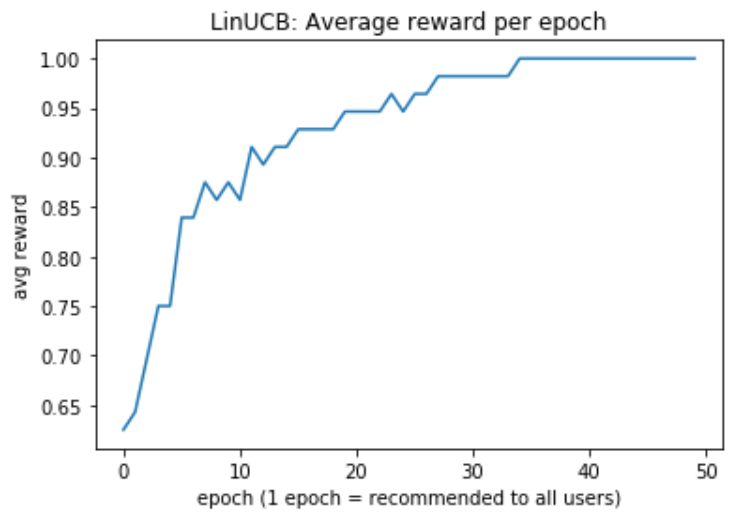
\includegraphics[width=\columnwidth]{img/LinUCB-100items-50epochs}
 \caption{LinUCB trained on 100 items and 56 users for 50 epochs.}
 \label{fig:linUCB}
\end{figure}

\begin{figure}[h]
 \centering
 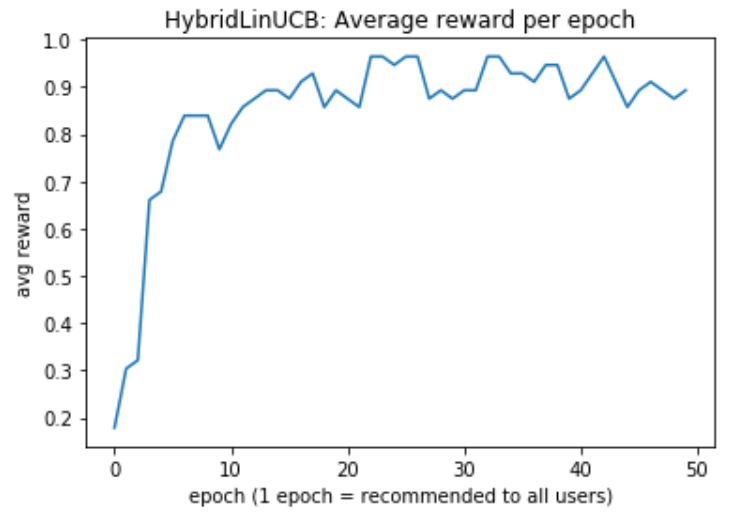
\includegraphics[width=\columnwidth]{img/HybridLinUCB-100items-50epochs}
 \caption{HybridLinUCB trained on 100 items and 56 users for 50 epochs.}
 \label{fig:linUCB}
\end{figure}









\end{document}